\documentclass[../main/thesis.tex]{subfiles}
\begin{document}
\newpage
%% my chapter 1 content
\chapter{Testing and Characterization of the 3DMiMic Detector}
\label{3dmimic}

\begin{figure}[h]
	\centering
	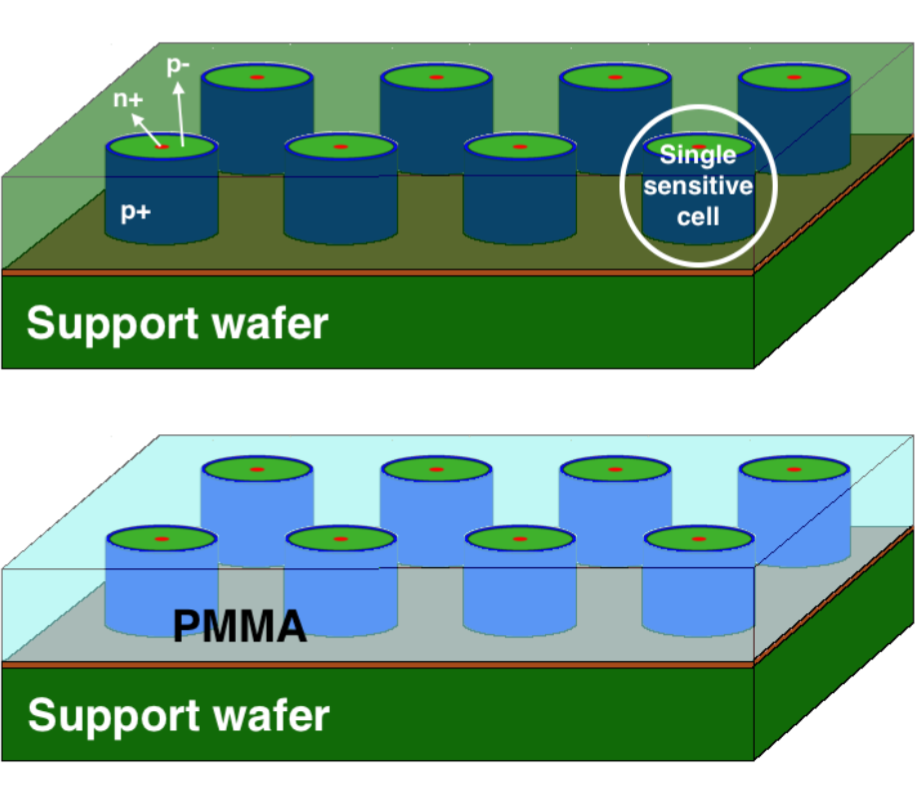
\includegraphics[width=0.6\textwidth]{3dmimic.png}
	\caption{Presentation sketches of the 3DMiMic detector, shown without and with PMMA. \citep{Trento2015}}
	\label{fig-3dmimic}
\end{figure}

\section{3DMiMic}
\label{3d-3d}
Si-3DMiMic, or simply 3DMiMic, is a silicon-based 3D mini and micro-dosimeter being developed by SINTEF MiNaLab in Oslo, but was invented and ordered by researchers at the University of Wollongong. The detector is made to mimic the response of biological tissues to ionizing radiation on a cellular and sub-cellular level, and consists of an array of 32x32 cylindrical p-i-n diodes. Each diode, or cell, is made of a thin n+ core cylinder (red in figure \ref{fig-3dmimic}), a circular p+ trench some micrometers out (dark blue in figure \ref{fig-3dmimic}), and in some cases a n+ ring further away from the core (to the right in figure \ref{fig-3dmimic-side}). There are multiple versions of the detectors, with differences including presence of n+ guard ring, size of cell, and structure. The silicon between the different cells should be etched away and replaced with tissue equivalent \gls{PMMA}, but this has not been attempted by SINTEF yet as of the time this thesis is written. This should be done because \gls{PMMA} is ionized by radiation very similar to the way tissue would, unlike silicon, due to the mass numbers of the atoms. 

%Each diode, or cell, is made of a 3 $\mu$m diameter n+ core cylinder, a 2 $\mu$m thick p+ trench about 10 $\mu$m further out, and a 4 $\mu$m thick n+ ring about 20 $\mu$m outside the core. The silicon between the different cells has been etched away and replaced with tissue equivalent \gls{PMMA}. %Need to double check all this later, I have contradicting sources

Figure \ref{fig-3dmimic-side} show a "3D" layout with the n+ core cylinder and the p+ trench going all the way through the bulk, and a planar n+ guard ring. There also exist designs with either or both the n+ core and p+ trench made planar. Figure \ref{fig-3dmimic-top15} shows the smallest, "15 $\mu$m", layout of 3DMiMic from above with a size scale. The larger, "30 $\mu$m", layout is roughly 25 \% larger than the "15 $\mu$m" layout. Images of some of the different layouts can be found in Appendix \ref{a-3dmimic-layout}.

\begin{figure}%[h]
	\centering
	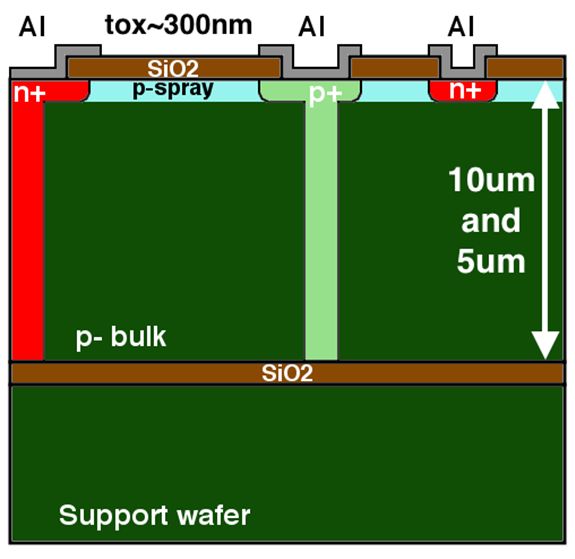
\includegraphics[width=0.5\textwidth]{3d-side.png}
	\caption{Layout of 3DMiMic design with 3D n+ core and 3D p+ trench. \citep{Marco}}
	\label{fig-3dmimic-side} %need to check permission
\end{figure}

\begin{figure}%[h]
	\centering
	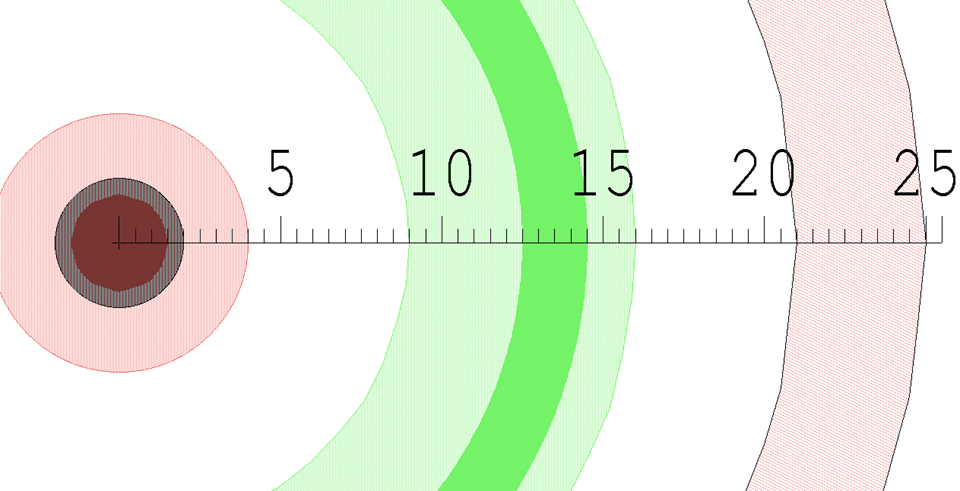
\includegraphics[width=0.6\textwidth]{3d-top15.png}
	\caption{Smallest, "15 $\mu$m", layout of 3DMiMic seen from above. Distance scale is in $\mu$m. \citep{Marco}}
	\label{fig-3dmimic-top15} %need to check permission
\end{figure}

In the main layout of 3DMiMic, all the n+ cores in a line is connected together. Every second line is also connected, leaving two channels (odd/even) for readout. When present, all the outer n+ rings are connected and can be read out if desired. There also exist other layouts, for example with all diodes connected together, readout in eight channels, and a larger design made to be bump bonded to a Medipix chip (see section \ref{e-medipix}). 

Even though the odd/even readout scheme contains two channels, it does not provide any spacial information, as both channels cover the whole active area of the detector. The reason for this layout is to notice if a particle track goes through multiple adjacent cells. If both readout channels are triggered at the same time, this was not a single event, as it will look if all cells are read in a single channel.

\section{I-V Measurements of 3DMiMic Detectors}
\label{3d-IV}
\gls{IV} measurements of seven 3DMiMic wafers where performed in the cleanroom at SINTEF MiNaLab in Oslo by Øyvind Lye and Andreas Tefre Samnøy in May 2016. These seven wafers have been produced with different designs and fabrication processes. Each wafer has 104 detectors with odd/even readout, 6 detectors with single channel readout, and several other experimental layouts. The detectors had to be tested with manual needle placement, as the designs are too different to use an automatic system with a probe card. The wafer is held in place on a stand using vacuum, and the stand can be moved in the horizontal plane. The needles can be manually placed at the desired location, and the position can be fine-tuned in Cartesian space using screws. The cell n+ guard ring was not connected on the detectors where it is present. This was done because it would require a separate test setup for the detectors with the ring, which would increase the time needed for the measurement. A total of 580 detectors were measured. 

\section{Detector Interface PCB}
\label{3d-pcb}
A \gls{PCB} was designed to interface 3DMiMic to the supply and readout electronics. This is described in more detailed in appendix \ref{a-pcb}.


\end{document}